\section{Applications}

\begin{frame}{Existing Applications}
There exist several applications of SPNs in various fields:
\begin{itemize}
    \item Computer vision, e.g.~image classification, medical image processing, attend-infer-repeat.
    \item Language processing, e.g.~language modelling, bandwidth extension.
    \item Robotics, e.g.~semantic mapping.
    \item Nonlinear regression, and many more\footnote{\scriptsize https://github.com/arranger1044/awesome-spn\#applications}
\end{itemize}
\end{frame}

\begin{frame}{SPNs for Regression}
We have recently\footnote{\scriptsize M. Trapp et al.: Deep structured mixtures of Gaussian processes. To appear at AISTATS, 2020.} introduced a combination of SPNs with Gaussian processes, which yields an interesting nonparametric regression model that allows exact and efficient posterior inference.

Our model can be understood as an exponentially large mixture over naive-local-experts of Gaussian processes.
\end{frame}

\begin{frame}{Deep Structured Mixtures of GPs}
    A Gaussian Process (GP) is a collection of random variables $F$ indexed by an arbitrary
    covariate space $X$, where any finite subset of $F$ is Gaussian distributed.

    A GP can be understood as a prior over functions.

    \begin{figure}
        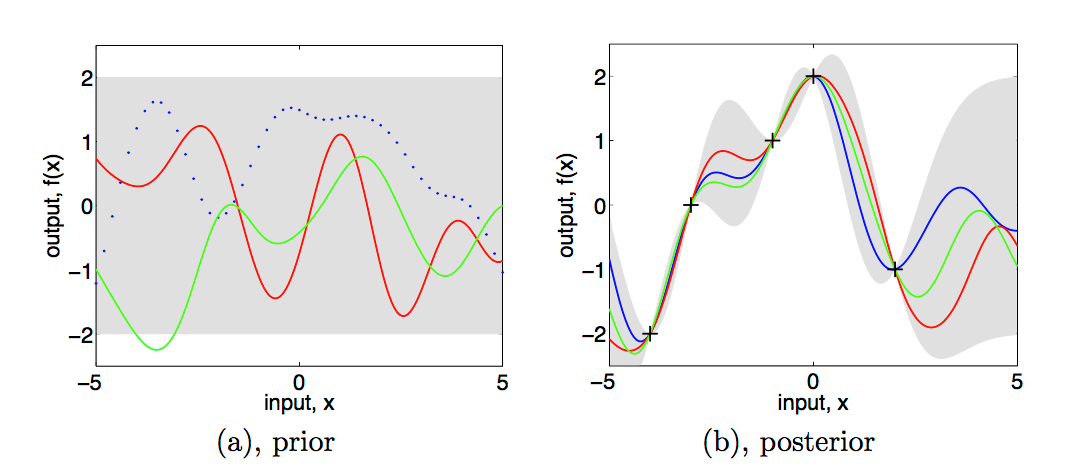
\includegraphics[width=0.9\textwidth]{GP_Rasmussen}
        \caption{\scriptsize C. E. Rasmussen \& C. K. I. Williams, Gaussian Processes for Machine Learning, 2006.}
    \end{figure}
\end{frame}
